\documentclass[a4paper, 12pt]{article}
\usepackage{cmap}
\usepackage{amssymb}
\usepackage{amsmath}
\usepackage{graphicx}
\usepackage{floatflt}
\usepackage{amsthm}
\usepackage{upgreek}
\usepackage{setspace}
\usepackage[T2A]{fontenc}
\usepackage[utf8]{inputenc}
\usepackage[normalem]{ulem}
\usepackage{arcs}
\usepackage{mathtext} % русские буквы в формулах
\usepackage[left=2cm,right=2cm, top=2cm,bottom=2cm,bindingoffset=0cm]{geometry}
\usepackage[english,russian]{babel}
\usepackage[unicode]{hyperref}
\newenvironment{Proof} % имя окружения
{\par\noindent{$\blacklozenge$}} % команды для \begin
{\hfill$\scriptstyle\boxtimes$}
\newenvironment{example} % имя окружения для примеров
{\par\noindent{\textsc{\textbf{Пример}.}}} % символ рядом с \begin
{\hfill$\scriptstyle\Box$} % символ рядом с \end
\newcommand{\Rm}{\mathbb{R}}
\newcommand{\Cm}{\mathbb{C}}
\newcommand{\Z}{\mathbb{Z}}
\newcommand{\I}{\mathbb{I}}
\newcommand{\N}{\mathbb{N}}
\newcommand{\p}{\prime}
\newcommand{\Ra}{\Rightarrow}
\newcommand{\ra}{\rightarrow}
\newcommand{\FI}{\Phi}
\newcommand{\Sp}{\text{Sp}}
\renewcommand{\leq}{\leqslant}
\renewcommand{\geq}{\geqslant}
\renewcommand{\alpha}{\upalpha}
\renewcommand{\beta}{\upbeta}
\renewcommand{\gamma}{\upgamma}
\renewcommand{\delta}{\updelta}
\renewcommand{\d}{\partial}
\renewcommand{\Re}{\operatorname{Re}}
\renewcommand{\Im}{\operatorname{Im}}
\newcommand{\Ln}{\operatorname{Ln}}
\newcommand{\Arccos}{\operatorname{Arccos}}
\newcommand{\intab}{\int\limits_a^b}
\newcommand{\intl}{\int\limits_l}
\newcommand{\Arcsin}{\operatorname{Arcsin}}
\renewcommand{\varphi}{\upvarphi}
\renewcommand{\tau}{\uptau}
\renewcommand{\rho}{\uprho}
\renewcommand{\lambda}{\uplambda}
\renewcommand{\psi}{\uppsi}
\renewcommand{\xi}{\upxi}
\newcommand{\sumz}{\sum\limits_{n = 0}^\infty }
\newcommand{\sumo}{\sum\limits_{n = 1}^\infty }
\renewcommand{\epsilon}{\upvarepsilon}
\newcommand{\limdef}{\forall \epsilon >0\ \exists \delta (\epsilon) > 0}
\newcommand\Norm[1]{\left\| #1 \right\|}
\newcommand\ef[1]{e^{i#1}}
\newcommand{\Arg}{\operatorname{Arg}}
\newtheorem*{theorem}{Теорема}
\newtheorem*{cor}{Следствие}
\newtheorem*{lem}{Лемма}
\title{\vspace{6.5cm}\textbf{\Huge{Теория функции комплексного переменного}}\\Конспект по 2 курсу 
	специальности «прикладная математика»\\(лектор А. А. Леваков)}
\date{}
\begin{document}
	\section*{Коллоквиум ТФКП.}
	\begin{enumerate}
		\item \begin{theorem}
			[о первообразной] Если функция $f(z)$ дифференцируема в односвязной области $D$, то функция $F(z) = \int\limits_{z_0}^z f(\zeta)d\zeta$ является первообразной в области $D$ для функции $f(z)$.
		\end{theorem}\begin{Proof}
			Возможность построения однозначной функции $F(z)$ вытекает из  следствия 1 интегральной теоремы Коши. Необходимо доказать, что $\forall z \in D$ $F'(z) = f(z)$. Возьмем точки $z$, $z + \Delta z \in D$. Тогда \begin{multline*}
				F'(z) = \lim\limits_{\Delta z \to 0} \dfrac{\Delta F(z)}{\Delta z} = \lim\limits_{\Delta z \to 0} \dfrac{F(z + \Delta z) - F(z)}{\Delta z} = \lim\limits_{\Delta z \to 0} \dfrac{\int\limits_{z_0}^{z + \Delta z}f(\zeta)d\zeta - \int\limits_{z_0}^{z}f(\zeta)d\zeta}{\Delta z}=\\=\text{[из независимости от формы пути]} = \lim\limits_{\Delta z \to 0} \dfrac{\int\limits_{z}^{z + \Delta z}f(\zeta)d\zeta}{\Delta z}.
			\end{multline*}
			\begin{multline*}
				F'(z) - f(z) = \lim\limits_{\Delta z \to 0}\Big(\dfrac{1}{\Delta z}\int\limits_{z}^{z + \Delta z}f(\zeta)d\zeta - f(z) \Big) = \lim\limits_{\Delta z \to 0}\Big(\dfrac{1}{\Delta z}\int\limits_{z}^{z + \Delta z}f(\zeta)d\zeta - \dfrac{f(z)}{\Delta z} \int\limits_{z}^{z + \Delta z}d\zeta \Big) = \\ =\lim\limits_{\Delta z \to 0} \dfrac{1}{\Delta z} \int\limits_{z}^{z + \Delta z} \Big( f(\zeta) - f(z)\Big)d\zeta = \Big[ \dfrac{1}{|\Delta z|}\cdot \Big|\int\limits_{z}^{z + \Delta z} \Big( f(\zeta) - f(z)\Big)d\zeta\Big|\leq \big[\\ \text{функция дифференцируема, следовательно, непрерывна в точке } z, \text{то есть} \\ \limdef \forall\zeta : |\zeta - z |\leq\delta (\epsilon) \Rightarrow |f(\zeta) - f(z)|\leq \epsilon \big] \leq \dfrac{1}{\Delta z}\epsilon\cdot |\Delta z| = \epsilon\Big] = 0.
			\end{multline*}
		\end{Proof}
	\item \begin{theorem}
		[о почленном дифференцировании степенного ряда]
		Если комплексный степенной ряд $\sumz c_nz^n$ имеет радиус сходимости $R>0$, то функция $f(z) =  \sumz c_nz^n$ является бесконечно дифференцируемой в круге $|z| < R$ и $m$-ая производная имеет вид $$f^{(m)}(z) = \sum\limits^\infty_{n = m} c_n \cdot n\cdot (n-1) \dots (n-m+1)\cdot z^{n-m},\ |z| < R, \forall m \in \N.$$
	\end{theorem}\begin{Proof}
		Рассмотрим ряд $S(z) = \sum\limits_{n=1}^\infty c_n\cdot n \cdot z^{n-1}$. Из формулы Коши-Адамара следует, что радиус сходимости этого ряда равен $$R_1 =  \dfrac{1}{\overline{\lim\limits_{n \to \infty}} \sqrt[n]{n\cdot |c_n|}} = R.$$
		Следовательно, ряд, сходящийся в функции, $S(z)$ имеет тот же радиус схожимости, что и ряд, сходящийся к $f(z)$.\\\\
		Возьмем окружность радиуса $\rho < R$. Тогда в круге $\overline{B}(0,\rho)$ ряд $\sum\limits_{n=1}^\infty c_n\cdot n \cdot z^{n-1}$ сходится равномерно по лемме Абеля. Возьмем произвольную точку $z$ и кривую $\gamma$, которая лежит в круге радиуса $\rho$ и соединяет точку $z$ с началом координат.$$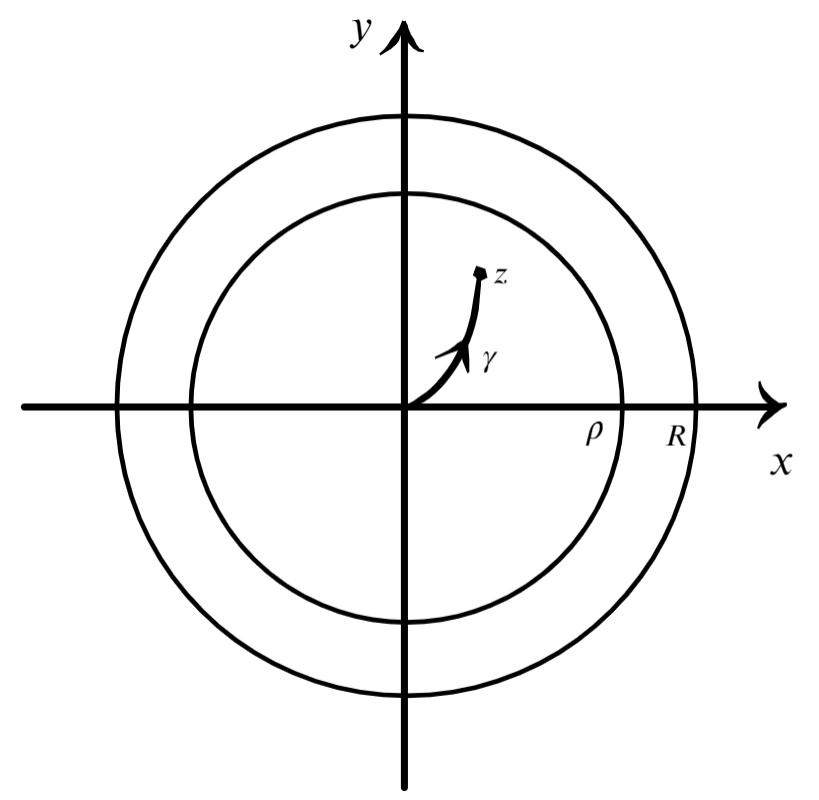
\includegraphics[scale=0.45]{images/034.png}$$ Тогда интеграл $\int\limits_\gamma z^{n-1}dz$ не зависит от кривой интегрирования, так как функ
		ция $z^{n-1}$ дифференцируема на всей плоскости. Следовательно, $$\int\limits_\gamma z^{n-1}dz = \int\limits_0^z \zeta ^{n-1}d\zeta = \dfrac{z^n}{n}.$$ Ряд $\sumo c_n\cdot n z^{n-1}$ сходится равномерно на кривой $\gamma$. Тогда по теореме о почленном интегрировании $$\int\limits_\gamma \sumo c_n\cdot n\cdot z^{n-1}dz = \sumo c_n\cdot n\cdot \dfrac{z^n}{n} = \sumo c_nz^n = f(z) - c_0.$$
		Причем интеграл слева не зависит от кривой интегрирования, следовательно $$\int\limits_0^z S(\zeta)d\zeta = f(z) - c_0.\eqno(1)$$
		Используя доказательство теоремы о первообразной, можно доказать, что $\int\limits_0^z S(\zeta)d\zeta$ --- первообразная для функции $S(z)$.\\\\
		Из равенства (1) получаем, что функция $f(z)$ является первообразной для функции $S(z)$. Значит $f'(z) = S(z)$. Отсюда функция $f(z)$ является дифференцируемой в круге $B(0,\rho)$. А так как $\rho$ можно вызять сколь угодно близким к $R$, то функция $f(z)$ дифференцируема в круге $B(0,R)$. Тогда $$f'(z) = \sumo c_n\cdot n\cdot z^{n-1}.$$
		Повторяя аналогичные рассуждения к функции $f'(z)$, можно показать, что через $(m-1)$ шагов получим $$f^{(m)}(z) = \sum\limits^\infty_{n = m} c_n \cdot n\cdot (n-1) \dots (n-m+1)\cdot z^{n-m}.$$
	\end{Proof}
\item \begin{theorem}
	[критерий регулярности функции в области]
	Функция $f(z)$ регулярна в области $D$ $\Longleftrightarrow$ функция $f(z)$ дифференцируема в области $D$.
\end{theorem}\begin{Proof}
	$\Rightarrow)$ Если функция регулярна в области, то она разложима в степенной ряд в этой области. А сумма комплексного степенного ряда --- функция дифференцируема по теореме о почленном дифференцировании степенного ряда.\\\\
	$\Leftarrow)$ Возьмем в области $D$ окружность $C(z_0,\rho)$ таким образом, чтобы она целиком лежала в области $D$. И возьмем произвольную точку $z$. $$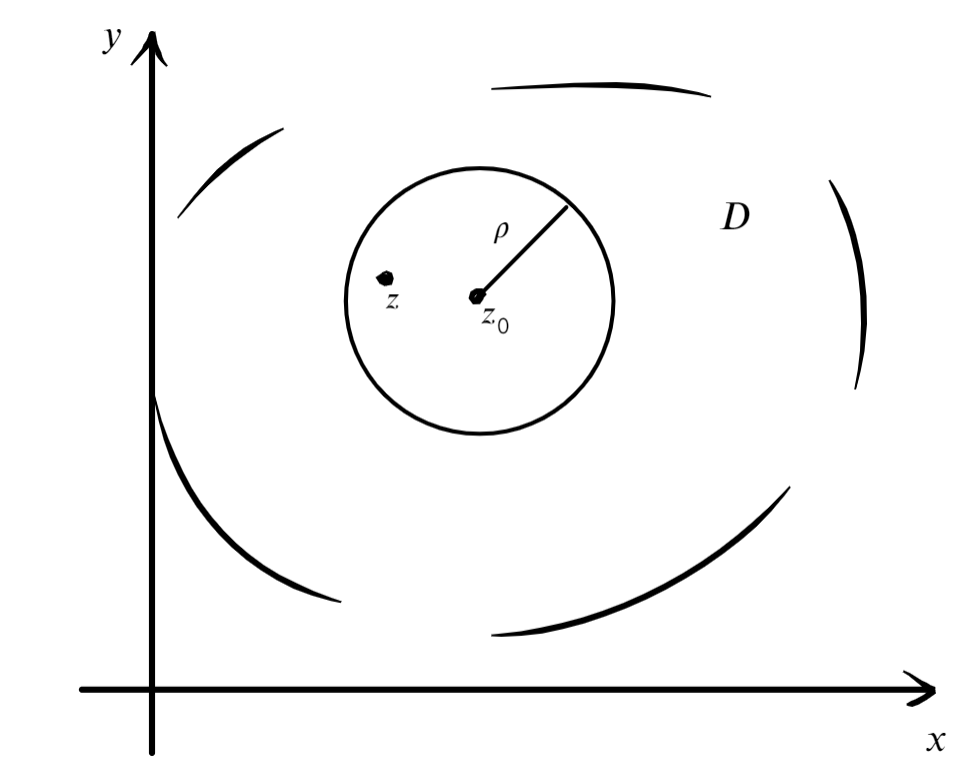
\includegraphics[scale = 0.45]{images/035.png}$$ Функция $f(z)$ дифференцируема в области $D$, значит дифференцируема и в окружности $C(z_0,\rho)$. По интегральной формуле Коши. $$f(z) = \dfrac{1}{2\pi i}\int\limits_{C(z_0,\rho)} \dfrac{f(\zeta)}{\zeta - z}d\zeta.$$
	Разложим в степенной ряд функцию $\dfrac{1}{\zeta - z}$ по степеням $z - z_0$:
	$$\dfrac{1}{\zeta - z} = \dfrac{1}{\zeta - z_0 + z_0 - z} = \dfrac{1}{(\zeta - z_0)(1 - \frac{z-z_0}{\zeta - z_0})} = \dfrac{1}{\zeta - z_0}\sumz\dfrac{(z-z_0)^n}{(\zeta - z_0)^n},$$
	Причем $\dfrac{|z-z_0|}{|\zeta - z_0|} < 1$. И пусть $\zeta \in C(z_0,\rho)$. Следовательно, ряд $\sumz\dfrac{(z-z_0)^n}{(\zeta - z_0)^n}$ сходится равномерно на окружности $C(z_0,\rho)$ по признаку Вейрштрасса.\\\\ Таким образом, ряд $$\dfrac{f(\zeta)}{\zeta - z} = \sumz \dfrac{f(\zeta)}{(\zeta - z_0)^{n+1}}(z-z_0)^n$$ также сходится равномерно на окружности $C(z_0,\rho)$.\\\\
	Проинтегрируем последнее равенство по окружности $C(z_0,\rho)$ и домножим обе части уравнения на $\dfrac{1}{2\pi i}$. Тогда $$\dfrac{1}{2\pi i}\int\limits_{C(z_0,\rho)} \dfrac{f(\zeta)}{\zeta - z}d\zeta = \sumz \dfrac{1}{2\pi i} \Big(\int\limits_{C(z_0,\rho)}\dfrac{f(\zeta)}{(\zeta - z_0)^{n+1}}d\zeta \Big)(z-z_0)^n = \sumz c_n(z-z_0)^n,$$
	где $$c_n = \dfrac{1}{2\pi i}\int\limits_{C(z_0,\rho)}\dfrac{f(\zeta)}{(\zeta - z_0)^{n+1}}d\zeta.$$
	Таким образом, $$f(z) =\sumz c_n(z-z_0)^n,\quad c_n = \dfrac{1}{2\pi i}\int\limits_{C(z_0,\rho)}\dfrac{f(\zeta)}{(\zeta - z_0)^{n+1}}d\zeta,\quad\forall z \in B(z_0, \rho).$$
\end{Proof}
\item \begin{theorem}
	[о представлении регулярной в кольце функции рядом Лорана]
	Если функция $f(z)$ регулярна в кольце $0\leq r < |z-z_0|<R$, то эта функция является суммой ряда Лорана, то есть $$f(z) = \sum\limits_{n=-\infty}^{+\infty}c_n(z-z_0)^n,$$ с коэффициентами $$c_n = \dfrac{1}{2\pi i}\int\limits_{C(z_0,\rho)}\dfrac{f(\zeta)}{(\zeta - z_0)^{n+1}}d\zeta,\quad r < \rho < R.$$
\end{theorem}\begin{Proof}
	Обозначим через $K$ кольцо $r < |z-z_0| < R$. Рассмотрим кривые $\Gamma$ и $\gamma$, лежащие в кольце $K$. Возьмем произвольную точку $z\in K$, лежащую между кривыми $\Gamma$ и $\gamma$.
	$$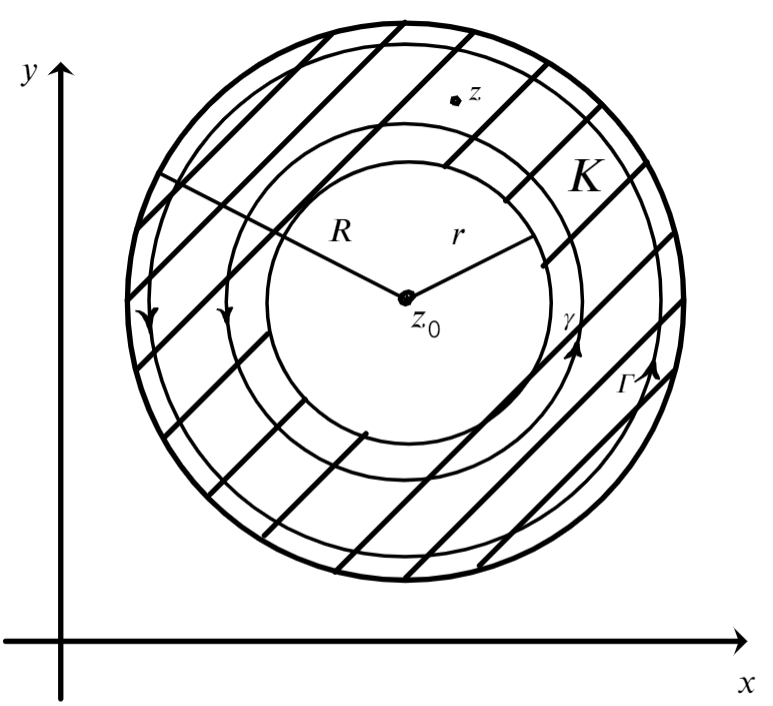
\includegraphics[scale=0.5]{images/041.png}$$
	По следствию 1 из интегральной формулы Коши $$f(z) =\dfrac{1}{2\pi i} \int\limits_{\Gamma} \dfrac{f(\zeta)}{\zeta-z_0}d\zeta - \dfrac{1}{2\pi i}\int\limits_{\gamma}\dfrac{f(\zeta)}{\zeta-z_0}d\zeta.$$
	Рассмотрим интеграл по $\Gamma$. По критерию регулярности $$\dfrac{1}{2\pi i} \int\limits_{\Gamma} \dfrac{f(\zeta)}{\zeta-z_0}d\zeta = \sumz c_n(z-z_0)^n.$$
	Отсюда $$c_n = \dfrac{1}{2\pi i}\int\limits_{\Gamma}\dfrac{f(\zeta)}{(\zeta - z_0)^{n+1}}d\zeta.$$
	Рассмотрим интеграл по $\gamma$. Разложим в степенной ряд функцию $-\dfrac{1}{\zeta - z}$ по степеням $z - z_0$: \begin{multline*}
		-\dfrac{1}{\zeta - z} = -\dfrac{1}{\zeta - z_0 + z_0 - z} =\dfrac{1}{(z-z_0) - (\zeta - z_0)}= \dfrac{1}{(z - z_0)(1 - \frac{\zeta-z_0}{z - z_0})}= \\=\sumz\dfrac{(\zeta-z_0)^n}{(z - z_0)^{n+1}} = [n+1 = -k] = \sum\limits_{k=-1}^{-\infty}\dfrac{(z-z_0)^k}{(\zeta - z_0)^{k+1}}.
	\end{multline*}
	Полученный ряд сходится равномерно на окружности $\gamma$ (это следует из леммы Абеля). Тогда ряд $$-\dfrac{f(\zeta)}{\zeta - z} = \sum\limits_{k=-1}^{-\infty}\dfrac{f(\zeta)}{(\zeta - z_0)^{k+1}}\cdot (z-z_0)^k$$
	также сходится равномерно на окружности $\gamma$. А так как $\gamma$ --- это компакт и функция $f(\zeta)$ непрерывна на этом компакте, то функция $f(\zeta)$ ограничена. Почленно проинтегрируем этот ряд: $$-\dfrac{1}{2\pi i}\int\limits_\gamma \dfrac{f(\zeta)}{\zeta - z}d\zeta = \dfrac{1}{2\pi i}\sum\limits_{n=-1}^{-\infty}\Big(\int\limits_\gamma\dfrac{f(\zeta)}{(\zeta - z_0)^{n+1}}d\zeta \Big)\cdot (z-z_0)^n= \sum\limits_{n=-1}^{-\infty} c_n(z-z_0)^n,$$
	где $$c_n = \dfrac{1}{2\pi i}\int\limits_\gamma  \dfrac{f(\zeta)}{(\zeta - z_0)^{n+1}}\cdot d\zeta.$$
	Таким образом, ряд Лорана имеет вид $$f(z) = \sumz\Big( \dfrac{1}{2\pi i}\int\limits_{\Gamma}\dfrac{f(\zeta)}{(\zeta - z_0)^{n+1}}d\zeta\Big)(z-z_0)^n + \sum\limits_{n=-1}^{-\infty}\Big(\dfrac{1}{2\pi i}\int\limits_\gamma\dfrac{f(\zeta)}{(\zeta - z_0)^{n+1}}d\zeta \Big)\cdot (z-z_0)^n.$$
	Возьмем окружность радиуса $\rho$. Обе кривые $\gamma$ и $\Gamma$ можно деформировать в эту окружность. Следовательно, вместо $\gamma$ и $\Gamma$ можно взять окружность радиуса $\rho$. 
	$$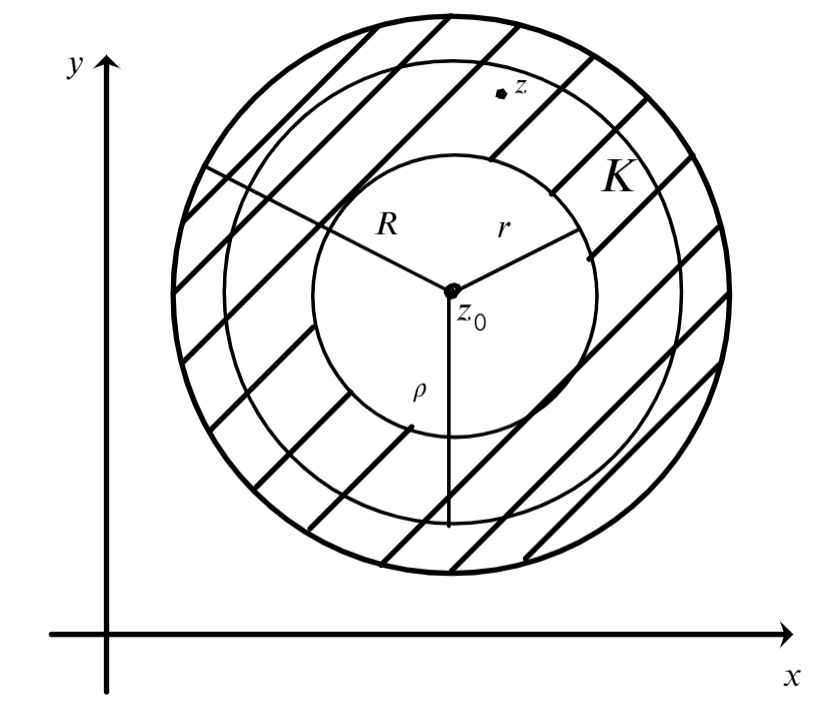
\includegraphics[scale = 0.5]{images/042.png}$$
	Тогда ряд Лорана можно записать в виде $$f(z) = \sum\limits_{n=-\infty}^{+\infty}c_n(z-z_0)^n,$$ с коэффициентами $$c_n = \dfrac{1}{2\pi i}\int\limits_{C(z_0,\rho)}\dfrac{f(\zeta)}{(\zeta - z_0)^{n+1}}d\zeta.$$ 
\end{Proof}
\item \begin{theorem}
	[об устранимой особой точке] Точка $z_0$ --- устранимая особая точка $\Longleftrightarrow$ главная часть разложения функции в ряд Лорана тождественно равна нулю.
\end{theorem}\begin{Proof}
	$\Rightarrow)$ Рассмотрим функцию $f(z)$ такую, что $z_0$ для нее --- устранимая особая точка. Докажем, что главная часть в разложении в ряд Лорана отсутствует. Берем ряд Лорана
	$$f(z) = \ldots + c_{-n}(z-z_0)^{-n} + \ldots + c_{-1}(z-z_0)^{-1} + c_0 + c_1(z-z_0) + \ldots + c_n(z-z_0)^n + \ldots.$$
	Точка $z_0$ --- устранимая особая точка, следовательно, $\exists \lim\limits_{z\to z_0} f(z) = A\in \Cm\Rightarrow$ функция $f(z)$ ограничена, то есть $\exists M : |f(z)|\leq M$ в круге $0 < |z-z_0| < \rho _1$. Воспользуемся неравенством для коэффициентов ряда Лорана:
	$$|c_n|\leq \dfrac{M}{R_0^n},\ M = \underset{z \in C(z_0,\rho)}{\max} |f(z)|,$$
	где $0 < R_0 < \rho_1$. Тогда $|c_{-n}| \leq MR_0^n$, но $R_0$ может быть сколь угодно близким к 0. Тогда, если $R_0\to 0$, то $MR_0^n \to 0$, следовательно, $c_{-n} = 0$, то есть все коэффициенты главной части ряда Лорана равны нулю, значит, главная часть равна нулю.\\\\
	$\Leftarrow)$ Пусть главная часть разложения в ряд Лорана функции $f(z)$ отсутствует, то есть в круге $0 < |z-z_0|<\rho$ $$f(z) = c_0 + c_1(z-z_0) +\ldots + c_n(z-z_0)^n + \ldots.$$
	Берем функцию $$g(z) = c_0 + c_1(z-z_0) +\ldots + c_n(z-z_0)^n + \ldots.$$ Тогда $f(z) = g(z)$ в кольце $0 < |z-z_0|<\rho$. И функция $g(z)$ определена и непрерывна в круге $|z-z_0| < \rho$ (в то время как $f(z)$ может быть и не определена). Следовательно, $$g(z_0) = A = \lim\limits_{z\to z_0} g(z) = \lim\limits_{z\to z_0}f(z).$$
\end{Proof}
	\end{enumerate}
\end{document}
